%\renewcommand{\lastmod}{\today}

\chapter{Schwingungsspektroskopie im Infraroten}

\label{chap:vib}

%https://webbook.nist.gov/cgi/cbook.cgi?ID=C74884&Type=IR-SPEC&Index=1#IR-SPEC

\section{Ziele}

\begin{itemize}
\item Sie können Vibrationsspektren von Molekülen in der Gasphase wie das untenstehende von HCN erklären und daraus Eigenschaften des Moleküls wie die  Federkonstante der Bindung oder die  Molekülform bestimmen.
\end{itemize}

%\tikzexternaldisable

\begin{figure}
\inputtikz{\currfiledir fig_hcn-single}
\caption{Infrarot-Absorptionsspektrum von HCN Gas  (\cite{Maki_1995_HCN} via \href{https://hitran.org}{hitran.org}).
\label{fig:vib_hcn}}
\end{figure}



\section{Wie misst man das ?}

Das Bindungspotential eines Moleküls kann in der Nähe des Minimums, also um den Gleichgewichts-Bindungsabstand $R_0$ herum, harmonisch genähert werden.
Wie wir in Kapitel \ref{chap:3_diel} schon abgeschätzt hatten hat die Federkonstante dieses harmonischen Potentials einen Wert von etwas $k \approx 200$~N/m. Damit ergibt sich eine Eigenfrequenz des harmonischen Oszillators von $\omega = \sqrt{k / m}$ die einer optischen Wellenlänge von etwa $\lambda \approx 5$~\textmu m oder einer Wellenzahl $\bar{\nu} \approx 2000$~cm$^{-1}$ entspricht. 

Absorptionsspektren in diesen (Nah-)Infraroten Wellenlängenbereich misst man beispielsweise durch Fourier-Transformations-Infrarot-Spektroskopie (FTIR). Als Lichtquelle wird oft ein breitbandiger Infrarotstrahler benutzt, der aus einem Silizium-Carbid-Stab (Globar) besteht, durch den ein Strom fließt und so heizt. Das durch die Probe transmittierte Licht wird durch ein Michelson-Interferometer geleitet und mit einem infrarot-  also Wärme-empfindlichen Detektor (Bolometer) gemessen. Dieser Detektor selbst kann nur die Gesamt-Intensität messen. Das Michelson-Interferometer wirkt aber als spektraler Filter mit einer sinusförmigen Transmission. Die Periode der spektralen Modulation wird über den Armlängen-Unterschied eingestellt und kontinuierlich variiert. Aus der Fourier-Transformation der gemessenen Intensität als Funktion des Armlängen-Unterschieds erhält man das Spektrum des Infrarot-Lichts, also Intensität als Funktion der Wellenlänge.



\section{Born-Oppenheimer-Näherung}

In der Schwingungsspektroskopie beobachtet man, dass sich im Molekül der Kern--Kern--Abstand  periodisch ändert, aber nicht durch irgendeine Art zeitaufgelöste Messung, sondern durch den Einfluss dieser Bewegung auf das Absorptionsspektrum. Das ist aber zunächst durch die Elektronen bestimmt, nicht die Kerne. Wir müssen in diesem Kapitel also sehr genau die Kerne und die Elektronen einerseits separieren und andererseits in ihrer Wechselwirkung betrachten. Dazu starten wir noch einmal mit der Born-Oppenheimer-Näherung, nun etwas formalisierter.

Das Molekül habe $N$ Elektronen der Masse $m$ am Ort $\mathbf{r}_i$ und $K$ Kerne des Masse $M_k$ am Ort $\mathbf{R}_k$. Die Vektoren $\mathbf{r}$ und $\mathbf{R}$ (\emph{ohne} Index) fassen \emph{alle} Koordinaten aller Elektronen bzw. Kerne zusammen, haben also eine sehr hohe Dimension, vereinfachen aber die Schreibweise. Die Schrödinger-Gleichung ist dann
\begin{equation}
 \hat{H} \, \Psi (\mathbf{r}, \mathbf{R}) = E \, \Psi (\mathbf{r}, \mathbf{R}) \quad \text{mit} \quad
  \hat{H} =  \hat{T}_e + \hat{T}_k + V (\mathbf{r}, \mathbf{R}) 
  \label{eq:vib_SG_allg}
\end{equation}
Die Operatoren $\hat{T}_{e,k}$ liefern die kinetische Energie und  $ V (\mathbf{r}, \mathbf{R}) $ \emph{alle} Coulomb-Potentiale, der Elektronen und Kerne untereinander und miteinander.

Falls die Kerne ruhen, also $\mathbf{R} = const.$, dann ist $\hat{T}_k = 0$. Wir betrachten jetzt die Bewegung der Kerne als Störung auf den Fall der ruhenden Kerne, also
\begin{equation}
 \hat{H} = \hat{H}_0 + \hat{H}' = \left( \hat{T}_e + V \right) +  \hat{T}_k
\end{equation}
Im ungestörten Fall lösen wir die Schrödinger-Gleichung
\begin{equation}
\hat{H}_0 \, \Phi_n^{el}  (\mathbf{r}, \mathbf{R})  = E_n^{(0)}  (\mathbf{R})  \, \Phi_n^{el}  (\mathbf{r}, \mathbf{R})    \label{eq:vib_SG_elec}
\end{equation}
In dieser Schreibweise ist $\mathbf{R}$ nur ein Parameter, der die stillstehende Kern-Positionen beschreibt. Weder differenzieren noch integrieren wir nach  $\mathbf{R}$. Die Lösungen der Schrödinger-Gleichung werden durch Quantenzahlen beschrieben, die hier alle in $n$ zusammengefasst sind. Die Eigenfunktionen $\Phi_n^{el}  (\mathbf{r}, \mathbf{R}) $ bilden ein vollständiges Orthonormalsystem, also können wir die eigentlich gesuchten $\Psi (\mathbf{r}, \mathbf{R})$ nach diesen entwickeln
\begin{equation}
\Psi (\mathbf{r}, \mathbf{R}) = \sum_m \chi_m (\mathbf{R}) \,\Phi_m^{el}  (\mathbf{r}, \mathbf{R}) 
\end{equation}
Die Koeffizienten $\chi_m (\mathbf{R}) $ sind die Kernwellenfunktionen. Zunächst setzen wir aber diesen Ansatz in die vollständige Schrödinger-Gleichung   \ref{eq:vib_SG_allg}ein und erhalten nach kurzer Rechnung\sidenote{siehe beispielsweise Kap. 2.1.2 in  \cite{Demtröder_molekuelphysik}}
\begin{equation}
\hat{H}' \, \chi_n (\mathbf{R}) + \sum_m \, c_{n m} \, \chi_m (\mathbf{R}) = \left( E - E_n^{(0)}(\mathbf{R})  \right) \chi_n (\mathbf{R})   \label{eq:vib_SG_kern}
\end{equation}
Die Kopplung der Kern-Wellenfunktionen $\chi_i (\mathbf{R}) $ ($i = m,n$) untereinander wird durch die Koeffizienten $c_{nm}$ beschrieben. Diese hängen von den Elektronenwellenfunktionen $\Phi_i^{el}  (\mathbf{r}, \mathbf{R}) $   ab. Die genaue Form von $c_{nm}$  wird hier nicht benötigt. Die beiden Gleichungen   \ref{eq:vib_SG_elec} und   \ref{eq:vib_SG_kern} bilden also ein gekoppeltes Gleichungssystem.

Die Born-Oppenheimer-Näherung entkoppelt dieses Gleichungssystem, in sie die Annahme macht
\begin{equation}
c_{n m } = 0
\end{equation}
Damit bleibt Gleichung \ref{eq:vib_SG_elec} unverändert und Gl. \ref{eq:vib_SG_kern} vereinfacht sich:
\begin{align}
\left( \hat{T}_e + V (\mathbf{r}, \mathbf{R}) \right) \, \Phi_n^{el}  (\mathbf{r}, \mathbf{R})  = &  \, E_n^{(0)}  (\mathbf{R})  \, \Phi_n^{el}  (\mathbf{r}, \mathbf{R})    \label{eq:vib_BO_el}\\
\left( \hat{T}_k + E_n^{(0)}(\mathbf{R})  \right) \, \chi_n (\mathbf{R}) =  &   \, E  \, \chi_n (\mathbf{R})   \label{eq:vib_BO_kern}
\end{align}
Dabei ist in Gl. \ref{eq:vib_BO_el} die Kernposition $\mathbf{R}$ nur als Parameter zu verstehen, in Gl. \ref{eq:vib_BO_kern} aber als Variable. Der Energie-Eigenwert der elektronischen Gleichung \ref{eq:vib_BO_el}  bildet das Potential für die Kernbewegung in Gleichung  \ref{eq:vib_BO_kern}, da er ja von der Position der Kerne abhängt. Die Elektronen wiederum bewegen sich in ihrem eigenen Coulomb-Potential und in dem der stillstehenden Kerne, beides in 
$V (\mathbf{r}, \mathbf{R}) $ zusammengefasst.


\section{Kernwellenfunktionen für zweiatomige Moleküle}

Wenn das Molekül nur aus zwei Atomen besteht, dann vereinfacht sich die Schrödinger-Gleichung für die Kernwellenfunktionen in der Born-Oppenheimer-Näherung beträchtlich. Wir starten von Gleichung \ref{eq:vib_BO_kern} und gehen in das Schwerpunktsystem der beiden Kerne. In die kinetische Energie $\hat{T}_k$ geht dann nur noch die reduzierte Masse und die Relativbewegung der Kerne ein, also ist $\mathbf{R}$ nur noch ein gewöhnlicher dreidimensionaler Vektor. Im Potential $ E_n^{(0)}(\mathbf{R})  $, das durch die Elektronen gebildet wird, geht sogar nur noch der Abstand der Kerne, also $R = |\mathbf{R}| $ ein, da die Orientierung der Kern--Kern--Achse für die Elektronen unwichtig ist. 

Alles zusammen ist dies also die Bewegung eines einzelnen Teilchens in einem sphärischen Potential, und damit formal äquivalent zum Wasserstoff-Atom, wenn auch mit einer anderen Potentialform. Analog zum Wasserstoff-Atom schreiben wir die Wellenfunktion $\chi$ als
\begin{equation}
 \chi (R, \theta, \phi) = \frac{U(R)}{R} \, Y_{l m} (\theta, \phi)
\end{equation}
Die Kugelflächenfunktionen $ Y_{l m} (\theta, \phi)$ geben die Winkelverteilung der Kernwellenfunktion an, die aus der im letzten Kapitel behandelten Rotation des Moleküls stammt. Wenn man dies alles in die Schrödinger-Gleichung für die Kernwellenfunktion einsetzt, vereinfacht sich diese zu
\begin{equation}
 \frac{d^2}{d R^2} U(R) + \frac{2 \mu }{\hbar^2} \left( E - E_n^{(0)}(R) - \frac{\hbar^2 J (J+1)}{2 \mu R^2} \right) U(R) = 0
 \label{eq:vib_zweiatom_U}
\end{equation}
Der letzte Term in der Klammer ist die Rotationsenergie der Kerne bei  Drehimpuls-Quantenzahl $J$ und reduzierter Masse $\mu$. Die Form des Bindungspotentials $E_n^{(0)}(R)$ bestimmt also $U(R)$ und damit die Kernwellenfunktion $\chi$.


\section{Harmonische Näherung des Bindungspotentials}

In der Nähe des Minimums, rund um den Gleichgewichtsabstand $R_0$ lässt sich das Bindungspotential sicherlich als harmonisches Potential nähern. Wir machen also die Annahme\sidenote{immer noch im zweiatomigen Molekül}
\begin{equation}
E_n^{(0)}(R)  = \frac{1}{2} \, k \, (R - R_0 )^2 = \frac{1}{2} \, k \, r^2 
\end{equation}
mit der Federkonstanten $k = \mu \, \omega_0^2$ und der Auslenkung $r$ aus dem Gleichgewicht. Weiterhin nehmen wir zunächst einmal an, dass das Molekül nicht rotiert, also $J=0$.  Damit wird Gl.\ref{eq:vib_zweiatom_U} zu
\begin{equation}
 \frac{d^2}{d \xi^2} U(\xi) + \left( \frac{2 E }{\hbar \omega_0}  - \xi^2  \right) U(\xi) = 0 \quad \text{mit} \quad \xi =  r \, \sqrt{\frac{\mu \omega_0}{\hbar}  }
\end{equation}
Diese Differentialgleichung wird gelöst durch die Schwingungs-Wellenfunktion des eindimensionalen harmonischen Oszillators
\begin{equation}
\Psi_\text{vib} =  U(\xi) = \left(\frac{\mu \omega_0}{\pi \hbar} \right)^{\frac{1}{4}} \,
 H_\nu(\xi) \, e^{- \xi^2 /2}
\end{equation}
mit den Hermite'schen Polynomen $H_\nu(\xi)$.
Die Energie-Eigenwerten sind
\begin{equation}
E_\nu = \hbar \omega_0 \left(\nu + \frac{1}{2} \right) \quad \text{mit} \quad \nu = 0, 1, 2 \dots
\end{equation}
und $\omega_0 = \sqrt{k / \mu}$. Die Aufenthaltswahrscheinlichkeit der Wellenfunktionen $\Psi_\text{vib}(r)$ fällt exponentiell wie $e^{-r^2}$ ab, falls $r \gg \sqrt{\hbar / \mu \omega_0}$. Die Hermite'schen Polylonem $H_\nu(\xi)$ haben $\nu$ Nullstellen. Dem Korrespondenzprinzip gehorchend ist die 
Aufenthaltswahrscheinlichkeit an den Umkehrpunkten des Oszillators besonders hoch, da dort klassisch ja die Geschwindigkeit Null ist.


\begin{marginfigure}
\inputtikz{\currfiledir vib_state_wf}
\caption{Die Eigenfunktionen des quantenmechanischen harmonischen Oszillators für $\nu = 0 \dots 5$ (dünne Linie) und die Aufenthaltswahrscheinlichkeit (gefüllte Kurven). Die Position in y-Richtung entspricht der Eigen-Energie des Zustands auf der Skala des parabelförmigen Bindungspotentials im Hintergrund.
\label{fig:vib_1d_WF}}
\end{marginfigure}


\section{Auswahlregeln für reine Schwingungsübergänge}

Lässt sich die Schwingung eines Moleküls (eigentlich der Kerne entlang der Bindungsachse) durch die Absorption eines Photons anregen? Oder andersherum: hinterlassen die Schwingungs-Energie-Eigenwerte $E_\nu$ von oben einen beobachtbaren Effekt? Hier wollen wir uns darauf beschränken, \emph{nur} die Schwingung anzuregen. Weiter unten werden wir Kombinationen mit anderen Anregungen (Rotation, Elektronisch) diskutieren.

Um diese Fragen zu beantworten hilft Fermis Goldene Regel zur Übergangsrate $\Gamma_{i \rightarrow f}$ vom Zustand $\ket{i}$ in den Zustand $\ket{f}$:
\begin{equation}
\Gamma_{i \rightarrow f} = \frac{2 \pi}{\hbar} \, |\braket{f | \hat{H}' | i} |^2 \, \rho(E_\textit{final})
\end{equation}
wobei $\hat{H}'$ den Stör-Operator beschreibt, der erst den Übergang verursacht, und $ \rho(E_\textit{final})$ die Dichte der Zustände, die erreicht werden können. Für optische Übergänge ist der Stör-Operator der Dipol-Operator, also
\begin{equation}
\hat{H}' = \hat{\mu} \cdot \mathbf{E}
\end{equation}
wobei hier $\mathbf{E}$ das elektromagnetische Feld am Ort des Moleküls beschreibt. Das Übergangsdipolmoment $\mathbf{D}_{fi}$ ist dann 
\begin{equation}
 \mathbf{D}_{fi} = \braket{f | \hat{\mu} | i} 
\end{equation}
und die Auswahlregeln beantworten die Frage, unter welchen Umständen dieser Term nicht Null ist und somit $\Gamma_{i \rightarrow f} $ nicht Null ist. Die absolute Größe interessiert uns hier also nicht so sehr.

In der vollständigsten Form bestehen die Wellenfunktionen aus dem elektronischen Anteil $ \Phi_n^{el}  (\mathbf{r}, \mathbf{R})  $, dem Kern-Rotations-Anteil $ Y_{l m} (\theta, \phi)$ und dem radialen Kern-Anteil  $\Psi_\text{vib}$. Da wir nur an reinen Schwingungs-Anregungen interessiert sind, reicht es hier aus, diesen letzten Anteil zu betrachten. Genauso besteht der Dipol-Operator eigentlich aus der Summe über alle Ladungen mal deren Ortsvektor. Auch dies vereinfacht sich zu dem Radialanteil der Kernladungen $d_k(R)$. Weiterhin nähern wir den Operator in einer Taylor-Reihe um $R \approx R_0$ und behalten nur das erste Glied. Die vollständige Rechnung findet sich in Kapitel 4.2 von \cite{Demtröder_molekuelphysik}. Dabei verschwindet auch das nullte Glied der Taylor-Reihe, das das statische Dipolmoment beschreibt. Man findet schließlich, dass das Übergangsmatrixelement gegeben ist durch
\begin{equation}
D_{fi}^\text{vib} \propto  \left. \frac{\partial d_k}{\partial R} \right|_{R_0} \,  \int (\Psi_\text{vib}^\star (R) )_f \, R  \, \, (\Psi_\text{vib} (R) )_i \, dR
\end{equation}
Reine Schwingungsübergang sind also nur dann erlaubt, wenn sich das permanente Dipolmoment mit dem Kern-Kern-Abstand ändert. Solche Moleküle werden infrarotaktiv genannt. Dann  darf auch das Integral nicht verschwinden. Aufgrund einer Eigenschaft der Hermite'schen Polynome ist das nur dann der Fall, wenn sich die Quantenzahl $\nu$ zwischen den beiden Zuständen nur um eins unterscheidet, also 
\begin{equation}
 \Delta \nu = \pm 1
\end{equation}
Reine Schwingungsübergänge sind also nur zwischen benachbarten Zuständen möglich, und das auch nur für manche Moleküle, bei denen sich das Dipolmoment mit dem Kern-Kern-Abstand ändert. \ch{NO} ist also infrarotaktiv, \ch{H2} nicht. Da im harmonischen Oszillator die Zustände äquidistant sind, bestehen reine Schwingungsspektren in diesem Fall aus einer einzigen Linie bei 
\begin{equation}
 \bar{\nu}_\text{vib} = \frac{\hbar \omega_0}{h c} = \frac{\sqrt{k / \mu} }{2 \pi  c}
\end{equation}

Das am Anfang des Kapitels gezeigte Spektrum ist deutlich komplexer. Unsere Annahme, dass sich allein die Schwingungs-Quantenzahl $\nu$ ändert, ist also (zu) weitreichend. Es wird sich zeigen, dass der scharfe Peak bei $\bar{\nu} = 715$~cm$^{-1}$ ein reiner Schwingungsübergang ist.

\section{Anharmonisches Bindungspotential}

Die harmonische Parabel ist nur eine erste Näherung für das Bindungspotential. Man kann verschiedene, besser zutreffende analytische Potentiale aufstellen. Oft wird das \emph{Morse-Potential} verwendet, weil auch mit ihm  die Schrödinger-Gleichung exakt lösbar ist. Das Potential habe die Form
\begin{equation}
 V(R) = D_e \left( 1 - e^{-a (R - R_0)} \right)^2 \approx D_e \, a^2 (R - R_0)^2 + \cdots
\end{equation}
Dabei ist $D_e$ die Dissoziationsenergie des Moleküls, also die Tiefe des Minimums unter der Energie bei $R \rightarrow \infty$. In der harmonischen Näherung des Morse-Potentials entspricht $k = 2 D_e a^2$ der Federkonstanten bzw. $\omega_0 = a \sqrt{2 D_e / \mu}$ der Eigenfrequenz. Als Energie-Eigenwerte erhält man
\begin{align}
 E_\nu =&  \hbar \omega_0 \left( \nu  + \frac{1}{2} \right)
 - \frac{\hbar^2 \omega_0^2}{4 D_e} \left( \nu  + \frac{1}{2} \right)^2 \\
 = &
 \hbar \omega_0 \left( \nu  + \frac{1}{2} \right)
 - \chi_e \, \hbar \omega_0  \left( \nu  + \frac{1}{2} \right)^2
\end{align}
mit der Anharmonizitätskonstanten $\chi_e =\hbar \omega_0 / 4 D_e$.
Die Zustände sind also nicht mehr äquidistant. Die Abstände zwischen benachbarten Zuständen nehmen mit steigender Quantenzahl $\nu$ ab. Die Auswahlregeln werden auch aufgeweicht, und Übergänge mit 
\begin{equation}
\Delta \nu = \pm 1, \pm 2 , \pm 3, \dots
\end{equation}
werden erlaubt, wenn auch sie mit steigendem $|\Delta \nu |$ schnell schwächer werden. Der spektroskopisch sichtbare Effekt des anharmonischen Bindungspotentials sind also die Obertöne, also Linien bei in etwa ganzzahligen Vielfachen der harmonischen Linie. Die Aufspaltung der harmonischen Linie selbst ist deutlich schwieriger zu beobachten. Für CO beispielsweise liegt der Grundton bei $\bar{\nu}_1 = 2142$~cm$^{-1}$ und der erste Oberton bei 
 $\bar{\nu}_2 = 4269$~cm$^{-1}$, aber $2 \bar{\nu}_1 = 4284$~cm$^{-1}$.
 
\begin{marginfigure}
\inputtikz{\currfiledir fig_vib_states}
\caption{Zustände und Übergange im harmonischen und anharmonischen Oszillator.}
\end{marginfigure}
 
 
 
Das anharmonische Bindungspotential erklärt auch die Expansion von Festkörpern --- eigentlich ein Thema für den dritten Abschnitt der Vorlesung. Der Schwerpunkt der Aufenthalts-Wahrscheinlichkeit der Schwingungs-Wellenfunktionen verschiebt sich mit steigender Quantenzahl im anharmonischen Oszillator zu größeren Bindungsabständen. Im harmonischen Oszillator bleibt er immer beim Gleichgewichtsabstand. Mit höherer Temperatur werden also immer höhere Schwingungszustände besetzt und so dehnt sich Materie aus.


\section{Rotation und Schwingung gleichzeitig}

Nun soll auch die Rotation des Moleküls erlaubt sein. Zunächst gehen wir davon aus, dass diese beiden Bewegungen sich nicht gegenseitig beeinflussen, also nicht gekoppelt sind. Die Energie-Eigenwerte sind dann gerade die Summe der Zustandsenergien aus Rotation und Schwingung\sidenote{Wir nehmen hier einen harmonischen Oszillator und einen starren Rotator an!}
\begin{equation}
E (\nu, J) = E_\text{vib}(\nu) + E_\text{rot}(J) = \hbar \omega_0 \left(\nu + \frac{1}{2} \right) + h c \, B J \left( J+1 \right) \label{eq:vib_rot_simple}
\end{equation}
mit der Rotations-Quantenzahl $J$ und der Vibrations-Quantenzahl $\nu$. Der energetische Abstand der Vibrationszustände ist mit etwa $1000$~cm$^{-1}$  größer als der der Rotationszustände mit etwa $100$~cm$^{-1}$. Man kann sich also vorstellen, dass nun jeder Schwingungszustand mit einer Sequenz von Rotationszuständen dekoriert ist.

Die Auswahlregeln sind zunächst dieselben wie wir sie bereits für die beiden Prozesse separat diskutiert hatten. Hinzu kommt die Möglichkeit, dass nichts passiert, also sich nur die andere Quantenzahl verändert. Damit haben wir
\begin{equation}
 \Delta \nu = 0, \pm 1 \quad \text{und} \quad \Delta J = 0, \pm 1 
\end{equation}
aber nicht alle Kombinationen sind möglich oder interessant.

\paragraph{Nichts passiert} Der Fall $\Delta \nu = \Delta J = 0$ ist langweilig.

\paragraph{Reine Rotationsübergänge} Falls $\Delta \nu = 0$ ändert sich nur der Rotationszustand. Dies ist die Situation, die wir im letzten Kapitel besprochen haben, und führt zu Linien  in einem anderen Spektralbereich, bei etwa $\bar{\nu} \approx 100$~cm$^{-1}$.

\paragraph{Reine Schwingungsübergänge} Am Anfang dieses Kapitel haben wir den  harmonischen Oszillator betrachtet unter der Annahme $J=0$. Dies schließt $\Delta J = 0$ mit ein. Bei einem von Null verschiedenen $J$ muss sich dieses aber bei einem Schwingungsübergänge ändern, zumindest für eine zweiatomiges Molekül. Eine höhere Schwingungsanregung ändert den mittleren Kern--Kern--Abstand und somit das Trägheitsmoment. Die Drehimpulserhaltung verlangt dann, dass sich die Rotationsquantenzahl $J$ ändert. $\Delta J = 0$ ist also verboten für einfache, zu symmetrische Moleküle, andernfalls erlaubt. Wenn diese Übergänge erlaubt sind, dann führen sie zu einer einzigen Linie im Spektrum bei $ \bar{\nu}_0 = (\hbar \omega_0)/(h c) $, analog dem reinen Schwingungsspektrum. Diese wird 'Q-Zweig' genannt. 

\paragraph{P-Zweig} Falls $\Delta J = -1$ ist, und $\Delta \nu = +1$ (in Absorption eines IR Photons) oder $-1$ (in Emission eines IR Photons), dann führen diese Übergänge zum sogenannten P-Zweig. Die Linienpositionen sind
\begin{equation}
 \frac{\Delta E}{h c} = \frac{1}{h c} \left( E(\nu +1, J -1) - E(\nu, J) \right) = \frac{\hbar \omega_0}{h c}   - 2 B J
\end{equation}
Wir erhalten also eine äquidistante Schar von Linien, völlig analog dem reinen Rotationsspektrum, insbesondere auch im dort besprochenen Verlauf der Amplituden. Der einzige Unterschied ist das negative Vorzeichen. Die Linienschar ist also gespiegelt gegenüber dem THz-Spektrum und beginnt an der reinen Schwingungslinie $\bar{\nu}_0 $.

\paragraph{R-Zweig} Analog zum P-Zweig, nur mit  $\Delta J = +1$ nur mit den Linienpositionen
\begin{equation}
 \frac{\Delta E}{h c} =  \bar{\nu}_0   + 2 B ( J +1)
\end{equation}
also in der gleichen Orientierung wie das THz-Spektrum und bei $\bar{\nu}_0 $ beginnend.

Mit diesen Überlegungen können wir das am Anfang des Kapitels gezeigte Spektrum zumindest qualitativ erklären.


\begin{marginfigure}
\inputtikz{\currfiledir rot_vib}
\caption{Rotations-Vibrations-Übergänge liefert die P, Q, R-Zweige im Spektrum.}
\end{marginfigure}
 
 
\section{Rotations-Schwingungs-Kopplung}

Bei der Diskussion des Q-Zweigs oben hatten wir ja schon den Fall, dass Rotation und Schwingung nicht unabhängig voneinander sind. Nur wenn diese koppeln kann der Q-Zweig erlaubt sein. Hier soll dies nun etwas detaillierter besprochen werden, und auch warum dies ein Q-Zweig und keine Q-Linie ist.

Im Molekül geschehen Rotation und Schwingung gleichzeitig, aber auf etwa um den Faktor 10 bis 100 verschiedenen Zeitskalen. Während einer Schwingungsperiode dreht sich das Molekül sehr oft. Das heißt aber auch, dass die Bindungslänge für die Rotation nicht konstant ist, sondern sich permanent ändert. Gleichzeit sind aber Gesamtenergie und Drehimpuls erhalten. Es muss also zu einem permanenten Austausch von Energie zwischen Rotation, Schwingung und Bindungspotential kommen. Was wir früher und auch weiterhin 'Rotationsenergie' nennen ist das zeitliche Mittel dieser Energie.

Um Gleichung \ref{eq:vib_rot_simple} zu verbessern, nehmen wir jetzt sowohl die Anharmonizität des Potentials als auch die Zentrifugaldehnung des Rotators mit in Betracht. Die Kopplung zwischen Rotation und Schwingung erfolgt dann über Rotationskonstanten, die von der Schwingungsquantenzahl $\nu$ abhängen
\begin{align}
 E(\nu, J) = & \hbar \omega_0 \left( \nu  + \frac{1}{2} \right)
 - \chi_e \, \hbar \omega_0  \left( \nu  + \frac{1}{2} \right)^2 \\
 & + h c \, B(\nu) J (J+1) - h c \, D(\nu) J^2 (J+1)^2  \nonumber
\end{align}
mit
\begin{equation}
B(\nu) = B_0 - \alpha \left(\nu + \frac{1}{2} \right) \quad \text{und} \quad
D(\nu) = D_0 + \beta \left(\nu + \frac{1}{2} \right) 
\end{equation}
Die (positiven) Koeffizienten $\alpha$ und $\beta$ beschreiben die  Rotations-Schwingungs-Kopplung. Das Vorreichen vor $\alpha$ ergibt sich aus der $\nu$-Abhängigkeit des mittleren Bindungsabstands $R$: dieser steigt mit $\nu$, wodurch das gemittelte $1/R^2$ und somit auch die gemittelte Rotationskonstante $B$ fällt, also $\alpha$ mit negativem Vorzeichen eingeht. Das Vorzeichen vor $\beta$ ist positiv, weil das anharmonische Bindungspotential mit $\nu$ weicher (also flacher) wird und so die Zentrifugalkraft einen größeren Einfluss auf die Rotation hat.

Alles zusammen rücken so die Linien im P-Zweig auseinander mit steigendem $J$, im R-Zweig rücken sie näher zusammen. Der Q-Zweig wird jetzt wirklich ein Zweig, da das anharmonische Potential ja nicht mehr äquidistante Zustände hat, $\Delta \nu = 1$ also mehrerer, aber eng benachbarte Linien liefert. Diese sind in der Abbildung am Anfang des Kapitels nicht aufgelöst.


\section{Mehratomige Moleküle}

Wenn ein Molekül aus mehr als zwei Atomen besteht, dann gibt es viele verschiedene, komplexe Muster der Auslenkung der einzelnen Atome aus ihrer Gleichgewichtsposition. Es gibt also mehr als eine Schwingungsmode in solchen Molekülen.

Die Anzahl der Schwingungsmoden lässt sich aus der Summe der Freiheitsgrade berechnen. Bei $N$ Atomen im Molekül hat jedes Atom $3$ Translations-Freiheitsgrade\sidenote{Atome sind hier punktförmig, können also nicht rotieren und haben daher keine Rotationsfreiheitsgrade}. Diese insgesamt $3N$ Freiheitsgrade müssen auch im Molekül existieren. Sie lassen sich aufteilen in
\begin{itemize} \setlength{\itemsep}{0pt}
\item Schwerpunktbewegung: 3 Freiheitsgrade
\item Rotation des Moleküls: 2 Freiheitsgrade, falls lineares Molekül, sonst 3 Freiheitsgrade
\item Schwingung: der ganze Rest, also $3N-5$ für ein lineares Molekül bzw. $3N-6$ für alle anderen Moleküle. 
\end{itemize}

Ein zweiatomiges Molekül wie beispielsweise \ch{H2} muss linear sein, hat also nur einen Schwingungs-Freiheitsgrad. Ein dreiatomiges Molekül kann linear sein, wie \ch{CO2} und hat dann 4  Schwingungs-Freiheitsgrade, oder es ist nicht gerade, wie \ch{H2O}, und hat dann nur 3  Schwingungs-Freiheitsgrade. Naphthalin beispielsweise besteht aus $N=18$ Atomen und hat damit  48 Schwingungs-Freiheitsgrade. Das Konzept der Normalmoden aus der Mechanik erlaubt hier den Überblick zu behalten.


\section{Normalmoden}

Wie handhabt man ein System aus $N$ Massen, die alle durch mehr oder weniger harmonische Potentiale miteinander verbunden sind? Dies ist ein Problem der klassischen Mechanik und führt zu den Normalmoden.\sidenote{siehe beispielsweise Kapitel 6.3 in \cite{Demtröder_molekuelphysik}}

Wir benutzen Masse-gewichtete generalisierte Koordinaten $q_i = \sqrt{m_i}  \Delta \tilde{q}_i$, wobei der Index $i$ über alle Atome und alle Raumrichtungen läuft, also von $1$ bis $3N$. $m_i$ ist die Masse des zugehörigen Atoms und 
$\Delta \tilde{q}_i$ die Auslenkung aus der Gleichgewichtsposition. Damit wird  die kinetische Energie $T$ 
\begin{equation}
T = \frac{1}{2} \sum_{i=1}^{3N} \dot{q}_i^2
\end{equation}
Für das Potential setzen wir eine Taylor-Reihe nach $q_i$ an. Wir legen den Nullpunkt der Energieskala auf das Minimum des Potentials. Damit verschwinden die ersten beiden Terme der Taylor-Reihe und wir behalten nur den nächsten
\begin{equation}
V \approx \frac{1}{2} \sum_{i,k = 1}^{3N} \frac{\partial V}{\partial q_i \partial q_k} \, q_i \, q_k = 
 \frac{1}{2} \sum_{i,k = 1}^{3N} b_{ik} \, q_i \, q_k 
\end{equation}
Damit können wir die Lagrange--Funktion $L = T - V$ bilden und erhalten in diesem Formalismus die Bewegungsgleichungen
\begin{equation}
 \ddot{q}_i + \sum_{k = 1}^{3N} b_{ik} \, q_k = 0 \quad \text{für} \quad i = 1 \dots 3N
\end{equation}
oder als Matrix mit $\tilde{\mathbf{B}} = (b_{ik})$ und $\mathbf{q} = (q_i)$
\begin{equation}
\ddot{\mathbf{q}} + \tilde{\mathbf{B}}  \cdot  \mathbf{q} = 0
\end{equation}
Dies ist ein System aus $3N$ gekoppelten Differentialgleichungen. Um sie zu entkoppeln diagonalisieren wir 
$\tilde{\mathbf{B}} $, suchen also $3N$ Eigenvektoren   $\mathbf{q}_n^0$ und (potentiell entartete) Eigenwerte $\lambda_n$ so dass
\begin{equation}
 \tilde{\mathbf{B}} \cdot \mathbf{q}_n^0 = \lambda_n \mathbf{q}_n^0 \quad \text{und damit} \quad
 \mathbf{q}_n(t) =  \mathbf{q}_n^0 \, e^{i \, t \, \sqrt{\lambda_n}}
\end{equation}
Die Eigenvektoren   $\mathbf{q}_n^0$ nennt man Normalmoden. Sie beschreiben also die gleichzeitige Bewegung aller Kerne in alle Raumrichtungen bei der Normal\-mode $n$ mit der Frequenz\sidenote{Manche $\lambda_n$ müssen Null sein, da es ja nur $3N - 5$ (oder 6) Normalmoden gebe kann.} $\omega_n = \sqrt{\lambda_n}$. Da die $b_{ik}$ reelwertig sind, schwingen in der Normalmode alle Atome in Phase, machen also gleichzeitig den Nulldurchgang, und natürlich mit der gleichen Frequenz. In der Basis der Normalmoden vereinfacht sich das Potential: es hat nur noch quadratische Formen der Art $\frac{1}{2} k q_i^2$ aber keine bi-linearen der Art $\frac{1}{2} k q_i q_k$, sonst wäre $\tilde{\mathbf{B}} $ ja nicht dialogisiert.

Die Normalmoden $\mathbf{q}_n^0$ sind komplexe Muster der Bewegung aller Atome. Man stellt diese grafisch dar, kann sie aber nicht als Achse in einem Diagramm verwenden. Dazu reduziert man weiter auf die Normalkoordinate
\begin{equation}
Q_n(t) = | \mathbf{q}_n (t) |
\end{equation}
also die masse-gewichtete Auslenkung aller Atome. Dieses $Q$ übernimmt in mehratomigen Molekülen die Rolle von $R$ im zweiatomigen Molekül. Die Energie einer Elementar-Anregung ist weiterhin 
\begin{equation}
E = \hbar \omega_n = \hbar	\sqrt{\lambda_n}
\end{equation}
Höhere Anregungen haben dann entsprechende Vielfache dieser Energie, und entsprechende Vielfache der Auslenkung 
 $\mathbf{q}_n^0$.


\section{Beispiele}

Wie kommt man an die Normalmoden? Das Aufstellen und Diagonalisieren der Matrix  $\tilde{\mathbf{B}} $ ist sicherlich unpraktikabel. Einen systematischen Weg bietet die Betrachtung der Symmetrie der Moleküle, die sich in der Symmetrie der Normalmoden widerspiegeln muss. Dies geschieht im Rahmen der Gruppentheorie, die hier allerdings zu weit gehen würde.\sidenote{Mehr dazu in der Vorlesung zur Kristallographie, oder qualitativ in \cite{Atkins}.} Hier raten wir einfach. Dabei hilft es, vorher auszurechnen, wie viele Moden man finden muss, also wie viele Schwingungsfreiheitsgrade es gibt. Auch sollte sich dabei der Schwerpunkt nicht bewegen, oder das ganze Molekül sich drehen, weil das ja separat behandelt wird.

\paragraph{Kohlendioxid} 
Ein lineares Molekül mit $f=9 - 5 = 4$ Schwingungsfreiheitsgraden


\begin{description}
\item[Symmetrische Streckschwingung]
\begin{marginfigure}
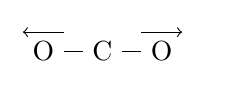
\begin{tikzpicture}
\useasboundingbox (-0.2,-0.2) rectangle (2,0.3);
%\draw (-0.2,-0.2) rectangle (2,0.3);

\draw  (0,0) node (o1) {O};
\draw  (0.75,0) node (c) {C};
\draw  (1.5,0) node (o2) {O};

\draw (o1) -- (c) -- (o2);
\draw[->] (o1.north east) -- (o1.north west);
\draw[<-] (o2.north east) -- (o2.north west);
\end{tikzpicture}
\end{marginfigure}
  $\bar{\nu} = 1337$~cm$^{-1}$. Hierbei ändert sich das Dipolmoment nicht, die Schwingung ist also nicht IR aktiv, wäre im Spektrum also nicht zu sehen.


\item[Asymmetrische Streckschwingung]
\begin{marginfigure}
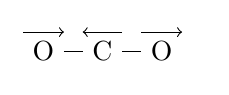
\begin{tikzpicture}
\useasboundingbox (-0.2,-0.2) rectangle (2,0.3);
%\draw (-0.2,-0.2) rectangle (2,0.3);

\draw  (0,0) node (o1) {O};
\draw  (0.75,0) node (c) {C};
\draw  (1.5,0) node (o2) {O};

\draw (o1) -- (c) -- (o2);
\draw[<-] (o1.north east) -- (o1.north west);
\draw[<-] (o2.north east) -- (o2.north west);
\draw[->] (c.north east) -- (c.north west);
\end{tikzpicture}
\end{marginfigure}
 $\bar{\nu} = 2349$~cm$^{-1}$. Hierbei ändert sich das Dipolmoment, die Schwingung ist also  IR aktiv.

\item[Biegeschwingung] 
\begin{marginfigure}
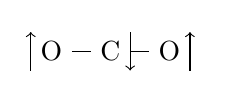
\begin{tikzpicture}
\useasboundingbox (-0.3,-0.2) rectangle (2,0.3);
%\draw (-0.2,-0.2) rectangle (2,0.3);

\draw  (0,0) node (o1) {O};
\draw  (0.75,0) node (c) {C};
\draw  (1.5,0) node (o2) {O};

\draw (o1) -- (c) -- (o2);
\draw[<-] (o1.north west) -- (o1.south west);
\draw[<-] (o2.north east) -- (o2.south east);
\draw[->] (c.north east) -- (c.south east);
\end{tikzpicture}
\end{marginfigure}
 $\bar{\nu} = 667$~cm$^{-1}$. Hierbei ändert sich das Dipolmoment, die Schwingung ist also  IR aktiv. Diese Mode ist zweifach entartet, da sie auch in der Ebene senkrecht zum Papier schwingen könnte. Für die Biegung ist das Potential weicher, die Frequenz daher niedriger als für die Streckung.
\end{description}


\paragraph{Wasser} Ein nicht-lineares Molekül mit $f=9 - 6 = 3$ Schwingungsfreiheitsgraden
\begin{description}
\item[Symmetrische Streckschwingung] 
\begin{marginfigure}
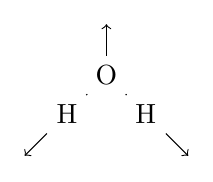
\begin{tikzpicture}
\useasboundingbox  (-0.5,-0.5) rectangle (1.5,1.1);
%\draw (-0.5,-0.5) rectangle (1.5,1.1);

\draw  (0,0) node (h1) {H};
\draw  (0.5,0.5) node (o) {O};
\draw  (1,0) node (h2) {H};

\draw (h1) -- (o) -- (h2);
\draw[->] (h1.south west) -- ++(-135:4mm);
\draw[->] (h2.south east) -- ++(-45:4mm);
\draw[->] (o.north) -- ++(up:4mm);
\end{tikzpicture}
\end{marginfigure}
  $\bar{\nu} = 3657$~cm$^{-1}$. Hierbei ändert sich das Dipolmoment, die Schwingung ist also  IR aktiv.

\item[Symmetrische Streck-Biegeschwingung]
\begin{marginfigure}
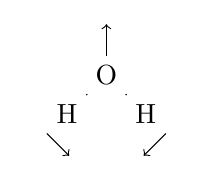
\begin{tikzpicture}
\useasboundingbox  (-0.5,-0.5) rectangle (1.5,1.1);
%\draw (-0.5,-0.5) rectangle (1.5,0.75);

\draw  (0,0) node (h1) {H};
\draw  (0.5,0.5) node (o) {O};
\draw  (1.,0) node (h2) {H};

\draw (h1) -- (o) -- (h2);
\draw[->] (h1.south west) -- ++(-45:4mm);
\draw[->] (h2.south east) -- ++(-135:4mm);
\draw[->] (o.north) -- ++(up:4mm);
\end{tikzpicture}
\end{marginfigure}
  $\bar{\nu} = 1595$~cm$^{-1}$. Hierbei ändert sich das Dipolmoment, die Schwingung ist also  IR aktiv.

\item[Asymmetrische Schwingung]
\begin{marginfigure}
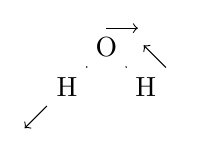
\begin{tikzpicture}
\useasboundingbox  (-0.5,-0.5) rectangle (1.5,0.75);
%\draw (-0.5,-0.5) rectangle (1.5,0.75);

\draw  (0,0) node (h1) {H};
\draw  (0.5,0.5) node (o) {O};
\draw  (1.,0) node (h2) {H};

\draw (h1) -- (o) -- (h2);
\draw[->] (h1.south west) -- ++(-135:4mm);
\draw[->] (h2.north east) -- ++(135:4mm);
\draw[->] (o.north) -- ++(east:4mm);
\end{tikzpicture}
\end{marginfigure}
  $\bar{\nu} = 3756$~cm$^{-1}$. Hierbei ändert sich das Dipolmoment, die Schwingung ist also  IR aktiv.
  
  
\end{description}

\paragraph{Cyanwasserstoff (Blausäure, HCN)}  
\begin{marginfigure}
\inputtikz{\currfiledir fig_hcn_modes}
\end{marginfigure}
Ein lineares Molekül mit $f=9 - 5 = 4$ Schwingungsfreiheitsgraden, analog zu Kohlendioxid oben. Das Spektrum am Anfang des Kapitels zeigt die Biegeschwingung bei $\bar{\nu} = 712$~cm$^{-1}$.  Abbildung \ref{fig:vib_hcn_all} gibt einen Überblick über einen größeren Spektralbereich. Man sieht zusätzlich den 
ersten Oberton der Biegeschwingung bei ungefähr der doppelten Frequenz  $\bar{\nu} = 1415$~cm$^{-1}$
. Die Mode bei  $\bar{\nu} = 3312$~cm$^{-1}$ ist die  asymmetrische Streckschwingung. Die symmetrische Streckschwingung  bei $\bar{\nu} = 2114$~cm$^{-1}$.
 Im Gegensatz zu \ch{CO2} bewegt sich in dieser Mode das Kohlenstoffatom ebenfalls, da die Massen von H und N verschieden sind, und sich ansonsten der  Schwerpunkt bewegen würde. Dies macht diese Mode sehr schwach IR-aktiv.  Nur für den Grundton der Biegeschwingung und die  symmetrische Streckschwingung ist der Q-Zweig erlaubt.

\begin{figure}
\inputtikz{\currfiledir fig_hcn-lowres}
\caption{Infrarot-Absorptionsspektrum von HCN Gas  (\cite{Maki_1995_HCN} via \href{https://hitran.org}{hitran.org}). Im unteren Spektrum ist ein größerer Ausschnitt bei geringer Auflösung gezeigt. Hier sind von den Rotationsbanden nur die Einhüllenden zu erkennen.
\label{fig:vib_hcn_all}}
\end{figure}








\printbibliography[segment=\therefsegment,heading=subbibliography]
